%
% abb.tex
%
% (c) 2018 Prof Dr Andreas Müller, Hochschule Rapperswil
%
\documentclass[tikz]{standalone}
\usepackage{times}
\usepackage{amsmath}
\usepackage{txfonts}
\usepackage[utf8]{inputenc}
\usepackage{graphics}
\usetikzlibrary{arrows,intersections,math}
\usepackage{ifthen}
\begin{document}

\newboolean{showgrid}
\setboolean{showgrid}{false}
\def\breite{8}
\def\hoehe{3}

\begin{tikzpicture}[>=latex,thick]

% Povray Bild
\node at (-3.2,0) {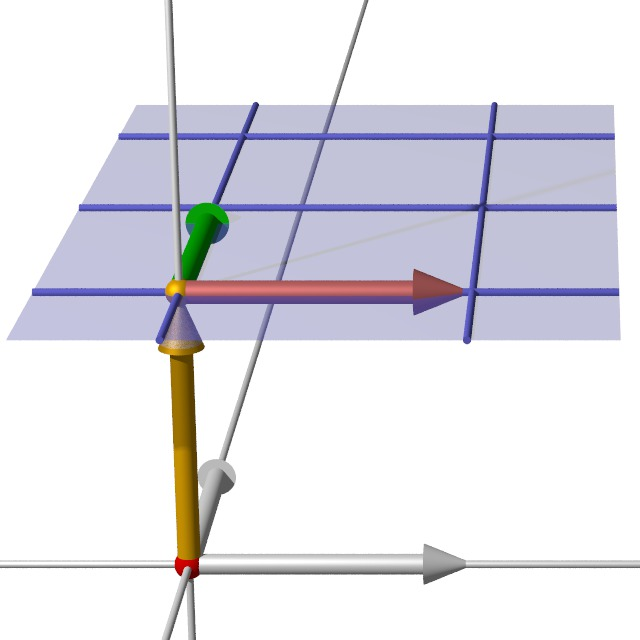
\includegraphics[height=5cm]{standardebene.jpg}};
\node at (5,0) {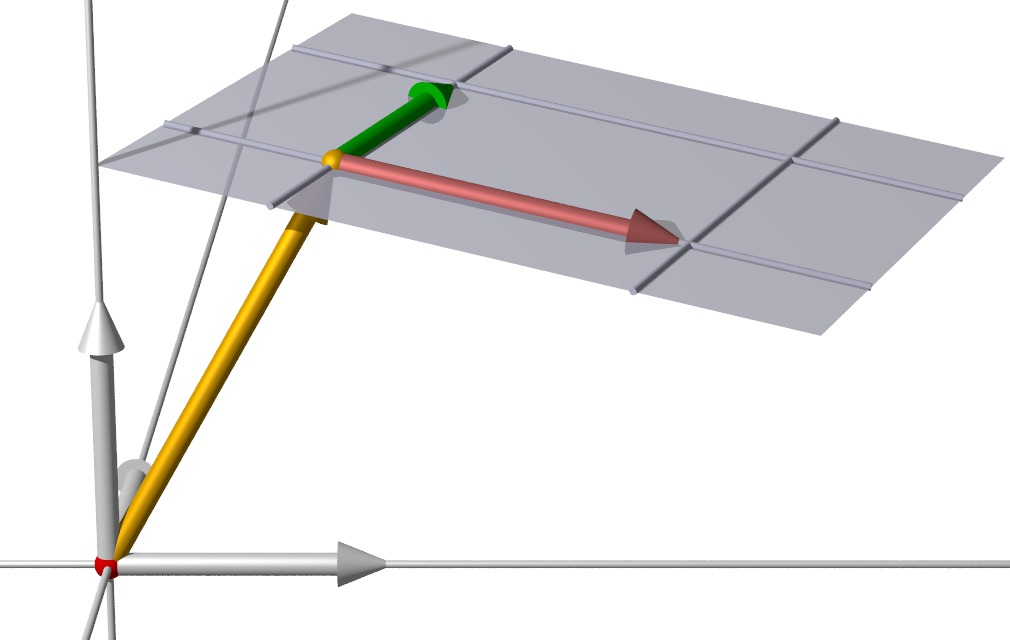
\includegraphics[height=5cm]{abbebene.jpg}};

% Gitter
\ifthenelse{\boolean{showgrid}}{
\draw[step=0.1,line width=0.1pt] (-\breite,-\hoehe) grid (\breite, \hoehe);
\draw[step=0.5,line width=0.4pt] (-\breite,-\hoehe) grid (\breite, \hoehe);
\draw                            (-\breite,-\hoehe) grid (\breite, \hoehe);
\fill (0,0) circle[radius=0.05];
}{}

% Legende links
\node at (-2.2,0.6) {$\vec{e}_1$};
\node at (-3.7,0.7) {$\vec{e}_2$};
\node at (-4.3,-0.9) [left] {$\vec{e}_3$};

% Legende rechts
\node at (2.8,-0.6) [right] {$\vec{p}$};
\node at (6.4,0.6) [above] {$\vec{u}$};
\node at (4.5,1.6) [right] {$\vec{v}$};

% Abbildungspfeil
\draw[->] (-0.6,0)--(1.4,0);
\node at (0.4,0) [above] {$A$};

\end{tikzpicture}

\end{document}

